\chapter{The Graph Abstract Data Type}
\label{ch:graphadt}

Many real-world applications, such as building compilers, finding routing
protocols in communication networks, and scheduling processes, are well
modelled using concepts from graph theory. A (directed) graph is an
abstract mathematical model:  a set of points and connection relations
between them.

\section{Basic definitions}
\label{sec:graphdefs}

Graphs can be studied from a purely mathematical point of view (``does
something exist, can something be done?"). In this book we focus on
algorithmic aspects of graph theory (``how do we do it efficiently and
systematically?").  However, the mathematical side is where we must
start, with precise definitions. The intuition behind the definitions is
not hard to guess.

We start with the concept of digraph (the word stands for
\textbf{di}rected \textbf{graph}). A good example to keep in mind 
is a street network with one-way streets. 

\begin{Definition}\label{def:digraph} 
A \defnfont{digraph} $G=(V,E)$ is a  finite nonempty set $V$ of
\defnfont{nodes} together with a (possibly empty) set $E$ of ordered pairs
of nodes of $G$ called \defnfont{arcs}.
\end{Definition}

\begin{note}   
In the mathematical language of relations, the definition says that
$E$ is a relation on $V$. If $(u, v)\in E$, we say that $v$ is \defnfont{adjacent} 
to $u$, that $v$ is an \defnfont{out-neighbour} of $u$, and that $u$ is an 
\defnfont{in-neighbour} of $v$.

We can think of a node as being a point and an arc as an arrow from one 
node to another. This allows us to draw pictures that suggest ideas. The 
pictures cannot \boldfont{prove} anything, however.
\end{note}

Very often the adjacency relation is symmetric (all streets are
two-way). There are two ways to deal with this. We can use a digraph
that happens to be symmetric (in other words, $(u, v)$ is an arc if and
only if $(v, u)$ is an arc). However, it is sometimes simpler to reduce
this pair of arcs into a single undirected edge that can be traversed in
either direction.

\begin{Definition}\label{def:graph}
A \defnfont{graph} $G=(V,E)$ is a finite nonempty  set $V$ of 
\defnfont{vertices} together with a (possibly empty) set $E$ of unordered
pairs of vertices of $G$ called \defnfont{edges}.
\end{Definition}

\begin{note}
Since we defined $E$ to be a set, there are no multiple arcs/edges
between a given pair of nodes/vertices.

Non-fluent speakers of English please note: the singular of ``vertices" is not
``vertice", but ``\defnfont{vertex}".

For a given digraph $G$ we may also denote the set of nodes by $V(G)$
and the set of arcs by $E(G)$ to lessen any ambiguity.
\end{note}

\begin{Example}
\label{eg:graphExample}
We display a graph $G_1$ and a digraph $G_2$ in
Figure~\ref{fig:graphExample}. The
nodes/vertices are labelled $0, 1, \dots $ as in the picture. The arcs
and edges are as follows.

$$E(G_1) = \set{\{0,1\},\{0,2\},\{1,2\},\{2,3\},\{2,4\},\{3,4\}}$$

$$E(G_2) = \set{(0,2),(1,0),(1,2),(1,3),(3,1),(3,4),(4,2)}$$


\begin{figure}
\centerline{\Ipe{./figs/graphEx.ipe}}
\caption{A graph $G_1$ and a digraph $G_2$.}
\label{fig:graphExample}
\end{figure}
\end{Example}

\begin{note} 
Some people like to view a graph as a special type of digraph where
every unordered edge $\{u,v\}$ is replaced by two directed arcs $(u,v)$
and $(v,u)$.  This has the advantage of allowing us to consider only
digraphs, and we shall use this approach in our Java implementation in Appendix~\ref{app:javagraph}. 
It works in most instances.

However, there are disadvantages; for some purposes we must know whether
our object is really a graph or just a symmetric digraph. Whenever there
is (in our opinion) a potential ambiguity, we shall point it out.
\end{note}

\begin{Example}
Every rooted tree (see Section~\ref{sec:app:trees}) 
can be interpreted as a digraph: there is an arc from
each node to each of its children. \index{rooted tree} 

Every free tree is a graph of a very special type (see
Appendix~\ref{sec:app:trees}). \index{free tree}
\end{Example}

\begin{note}(Graph terminology)
The terminology in this subject is unfortunately not completely
standard. Some authors call a graph by the longer term ``undirected
graph'' and use the term ``graph" to mean what we call a directed graph.
However when using our definition of a graph,  it is standard practice
to abbreviate the phrase ``directed graph'' with the word digraph.


We shall be dealing with both graphs and digraphs throughout these
notes. In order to save writing ``(di)graph" too many times, we make the
following convention.  We treat the digraph as the fundamental concept.
In other words, we shall use the terminology of digraphs, nodes and
arcs, with the understanding that if this is changed to graphs, edges,
and vertices, the resulting statement is still true. However, if we talk
about graphs, edges, and vertices, our statement is not necessarily true
for digraphs. Whenever a result is true for digraphs but not for graphs,
we shall say this explicitly (this happens very rarely).  

There is another convention to discuss. An arc that begins and ends at the
same node is called a \defnfont{loop}. We make the convention that
\boldfont{loops are not allowed in our digraphs}. Again, other authors
may differ. If our conventions are relaxed to allow multiple arcs and/or
loops, many of the algorithms below work with no modification or with only
very minor modification required. However dealing with loops frequently
requires special cases to be considered, and  would distract us from our
main goal of introducing the field of graph algorithms. As an example
of the problems caused by loops, suppose that we represent a graph as
a symmetric digraph as described above. How do we represent a loop in
 the graph?
\end{note}


\begin{Definition} 
The \defnfont{order} of a digraph $G=(V,E)$ is $|V|$, the number of nodes. 
The \defnfont{size} of $G$ is $|E|$, the number of arcs.

\end{Definition}
 
We usually use $n$ to denote $|V|$ and $m$ to denote
$|E|$.

For a given $n$, the value of $m$ can be as low as $0$ (a digraph
consisting of $n$ totally disconnected points)  and as high as
$n(n-1)$ (each node can point to each other node; recall that we do
not allow loops). If $m$ is toward the low end, the digraph is called
\defnfont{sparse}, and if $m$ is toward the high end, then the digraph
is called \defnfont{dense}. These terms are obviously very informal. For
our purposes we will call a class of digraphs sparse if $m$ is $O(n)$
and dense if $m$ is $\Omega(n^2)$.

\begin{Definition} 
A \defnfont{walk} in a digraph $G$ is a sequence of nodes $v_0\, v_1\,
\ldots\, v_l$ such that, for each $i$ with $0 \leq i < l$, $(v_i,
v_{i+1})$ is an arc in $G$. The \defnfont{length} of the walk $v_0\, v_1\,
\ldots \,v_l$ is the number $l$ (that is, the number of arcs involved).

A \defnfont{path} is a walk in which no node is repeated. A
\defnfont{cycle} is a walk in which $v_0 = v_l$ and no other nodes
are repeated.
\end{Definition}

Thus in a graph, we rule out a walk of the form $u\, v\, u$ as a
cycle (going back and forth along the same edge should not count as a
cycle). A cycle in a graph must be of length at least $3$.

It is easy to see that if there is a walk from $u$ to $v$, then
(by omitting some steps if necessary) we can find a path from $u$ to $v$.


\begin{Example}
For the graph $G_1$ of Figure~\ref{fig:graphExample} the following
sequences of vertices are classified as being walks, paths, or cycles.

\medskip

\begin{center}
\begin{tabular}{|l|c|c|c|}\hline
\textbf{vertex sequence} & \textbf{walk?} & \textbf{path?} & \textbf{cycle?} \\ \hline
$0\, 3\, 2$ & no & no & no  \\
$0\, 1\, 2\, 3\, 4$ & yes & yes & no  \\
$0\, 1\,  2\,  0$ & yes & no & yes  \\
$1\,  2\,  3\,  4\,  2\,  0$ & yes & no & no \\
$0 \, 1\,  0$ & yes & no & no \\
\hline
\end{tabular}
\end{center}
\end{Example}


\begin{Example}
For the digraph $G_2$ of Figure~\ref{fig:graphExample} the following
sequences of nodes are classified as being walks, paths, or cycles.

\medskip


\begin{center}
\begin{tabular}{|l|c|c|c|}\hline
\textbf{node sequence} & \textbf{walk?} & \textbf{path?} &
\textbf{cycle?} \\ \hline
$0\,  1\,  2\,  3\,  4$ & no & no & no  \\
$3\,  1\,  2$ & yes & yes & no \\
$1\,  3\,  1$ & yes & no & yes \\
$1\, 3\, 1\, 2$ & yes & no & no \\
$0\,  2\,  4$ & no & no & no \\
\hline
\end{tabular}
\end{center}
\end{Example}


\begin{Definition} 
In a graph, the \defnfont{degree} of a vertex $v$ is the number of edges
meeting $v$. In a digraph, the \defnfont{outdegree} of a node $v$ is the
number of out-neighbours of $v$, and the \defnfont{indegree} of $v$ is the
number of in-neighbours of $v$.

A node of indegree $0$ is called a \defnfont{source} and a node of outdegree $0$ is called a \defnfont{sink}.
\end{Definition}

If the nodes have a natural order, we may simply list the indegrees or
outdegrees in a sequence.

\begin{Example}
For our graph $G_1$, the degree sequence is $(2, 2, 4, 2, 2)$.
The in-degree sequence and out-degree sequence of the digraph $G_2$ are
$(1,1,3,1,1)$ and $(1,3,0,2,1)$, respectively. Node $2$ is a sink.
\end{Example}


\begin{Definition}
The \defnfont{distance} from $u$ to $v$ in $G$, denoted by $d(u,v)$, is 
the minimum length of a path from $u$ to $v$. If no path exists, the 
distance is undefined (or $+\infty$).
\end{Definition}

For graphs, we have $d(u,v) = d(v,u)$ for all vertices $u, v$. 

\begin{Example}
In graph $G_1$ of Figure~\ref{fig:graphExample}, we can see by considering
all possibilities that $d(0, 1) = 1$, $d(0, 2) = 1$, $d(0, 3) = 2$,
$d(0, 4) = 2$, $d(1, 2) = 1$, $d(1, 3) = 2$, $d(1, 4) = 2$, $d(2, 3) =
1$, $d(2, 4) = 1$ and $d(3, 4) = 1$.

In digraph $G_2$, we have, for example, $d(0, 2) = 1, 
d(3, 2) = 2$. Since node $2$ is a sink, $d(2, v)$ is not defined 
unless $v = 2$, in which case the value is $0$.

\end{Example}



There are several ways to create new digraphs from old ones.

One way is to delete (possibly zero) nodes and arcs in such a way that the 
resulting object is still a digraph (there are no arcs missing any
endpoints!).

\begin{Definition}
A \defnfont{subdigraph} of a digraph $G = (V, E)$ is a digraph $G' = (V', E')$ 
where $V'\subseteq V$ and $E'\subseteq E$. A \defnfont{spanning} subdigraph 
is one with $V'=V$; that is, it contains all nodes.
\end{Definition}

\begin{Example}
Figure~\ref{fig:sub+span} shows (on the left) a subdigraph and (on the right) 
a spanning subdigraph of the digraph $G_2$ of Figure~\ref{fig:graphExample}.
\end{Example}

\begin{figure}[h]
\begin{center}
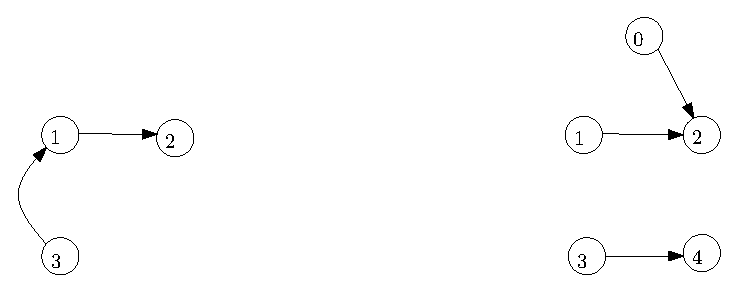
\includegraphics[width=4in]{figs/wSub+Span.eps}
\end{center}
\caption{A subdigraph and a spanning subdigraph of $G_2$.}
\label{fig:sub+span}
\end{figure}

\begin{Definition}
The subdigraph \defnfont{induced} by a subset $V'$ of $V$ is the digraph
$G' = (V', E')$ where $E' = \set{(u, v) \in E \mid u \in V' \mbox{ and } v\in V'}$.
\end{Definition}

\begin{Example}
Figure~\ref{fig:induced} shows the subdigraph of the  digraph $G_2$ of Figure~\ref{fig:graphExample} induced by 
\set{1, 2, 3}.
\end{Example}

\begin{figure}[h]
\begin{center}
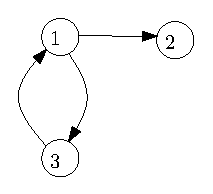
\includegraphics{figs/wInduced.eps}
\end{center}
\caption{The subdigraph of $G_2$ induced by \set{1, 2, 3}.}
\label{fig:induced}
\end{figure}

We shall sometimes find it useful to ``reverse all the arrows''.

\begin{Definition}
The \defnfont{reverse digraph} of the digraph $G = (V, E)$, is the digraph $G_r = (V, E')$ where $(u, v)\in E'$ if and only if $(v, u)\in E$.
\end{Definition}

\begin{Example}
Figure~\ref{fig:reverse} shows the reverse of the digraph $G_2$ of Figure~\ref{fig:graphExample}.
\end{Example}

\begin{figure}[h]
\begin{center}
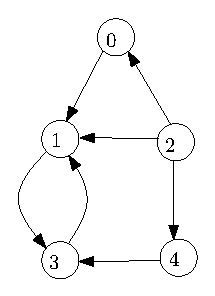
\includegraphics{figs/wReverse.eps}
\end{center}
\caption{The reverse of digraph $G_2$.}
\label{fig:reverse}
\end{figure}

It is sometimes useful to replace all one-way streets with two-way
streets. The formal definition must take care not to introduce multiple
edges. Note below that if $(u, v)$ and $(v, u)$ belong to $E$, then only
one edge joins $u$ and $v$ in $G'$.  This is because $\{u, v\}$ and
$\{v, u\}$ are equal as sets, so appear only once in the set $E'$.

\begin{Definition}
The \defnfont{underlying graph} of a digraph $G = (V, E)$ is the graph 
$G' = (V, E')$ where $E' = \set{\{u, v\} \mid (u, v)\in E}$.
\end{Definition}

\begin{Example}
Figure~\ref{fig:underly} shows the underlying graph of the digraph 
$G_2$ of Figure~\ref{fig:graphExample}.
\end{Example}

\begin{figure}
\begin{center}
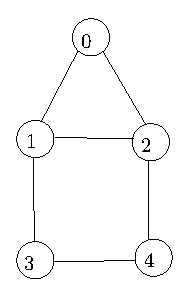
\includegraphics{figs/wUnderly.eps}
\end{center}
\caption{The underlying graph of $G_2$.}
\label{fig:underly}
\end{figure}

We may need to combine two or more digraphs $G_1, G_2$, \ldots $G_k$ into a
single graph where the vertices of each $G_i$ are completely disjoint from
each other and no arc goes between the different $G_i$. The constructed
graph $G$ is called the \defnfont{graph union}, where $V(G) = V(G_1) \cup
V(G_2) \cup \ldots \cup V(G_k)$ and $E(G) = E(G_1) \cup E(G_2) \cup \ldots
\cup E(G_k)$.

\subsection*{Exercises}

\begin{Exercise}
\label{ex:degree}
Prove that in a digraph, the sum of all outdegrees equals the sum of all 
indegrees. What is the analogous statement for a graph? 
\end{Exercise}

\begin{Exercise}
\label{ex:distbound}
Let $G$ be a digraph of order $n$ and $u, v$ nodes of $G$. 
Show that $d(u, v) \leq n - 1$ if there is a walk from $u$ to $v$.
\end{Exercise}


\begin{Exercise}
\label{ex:sparse-deg}
Prove that in a sparse digraph, the average indegree of a node is
$O(1)$, while in a dense digraph, the average indegree of a node is
$\Omega(n)$.
\end{Exercise}

\section{Digraphs and data structures}\label{sec:graph-reps}

In order to process digraphs by computer we first need to consider how
to represent them in terms of data structures. There are two common
computer representations for digraphs, which we now present. We assume
that the digraph has the nodes given in a fixed order. Our
\boldfont{convention} is that the vertices are labelled $0, 1, \dots, n - 1$.

\begin{Definition}
Let $G$ be a digraph of order $n$. The \defnfont{adjacency matrix} of $G$
is the $n\times n$ boolean matrix (often encoded with $0$'s and $1$'s)
such that entry $(i,j)$ is true if and only if there is an arc from the
node $i$ to node $j$.
\end{Definition}

\begin{Definition}
For a digraph $G$ of order $n$, an \defnfont{adjacency lists}
representation is a sequence of $n$ sequences, $L_0, \dots, L_{n-1}$. 
Sequence $L_i$  contains all nodes of $G$ that are adjacent to node $i$.
\end{Definition}

The sequence $L_i$ may or may not be sorted in order of increasing node number. 
Our \boldfont{convention} is to sort them whenever it is convenient.
(However, many implementations, such as the one given in
Appendix~\ref{app:javagraph}, do \emph{not} enforce that their 
adjacency lists be sorted.)

We can see the structure of these representations more clearly with
examples.

\begin{Example}
For the graph $G_1$ and digraph $G_2$ of Example~\ref{eg:graphExample}, 
the adjacency matrices are given below.
$$
G_1: 
\left[
\begin{matrix}
0 & 1 & 1 & 0 & 0 \\
1 & 0 & 1 & 0 & 0 \\
1 & 1 & 0 & 1 & 1 \\
0 & 0 & 1 & 0 & 1 \\
0 & 0 & 1 & 1 & 0 
\end{matrix}
\right]
\qquad 
G_2: 
\left[
\begin{matrix}
0 & 0 & 1 & 0 & 0 \\
1 & 0 & 1 & 1 & 0 \\
0 & 0 & 0 & 0 & 0 \\
0 & 1 & 0 & 0 & 1 \\
0 & 0 & 1 & 0 & 0 
\end{matrix}
\right]
$$

Notice that the number of $1$'s in a row (column) is the outdegree
(indegree) of the corresponding node. The corresponding adjacency lists 
are now given.

\begin{center}
$$
G_1: \quad
\AdjLists{
\begin{array}{cccc}
1 & 2  \\
0 & 2 \\
0 & 1 & 3 & 4  \\
2 & 4  \\
2 & 3  \\
\end{array}
}
\qquad
G_2: 
\quad 
\AdjLists{
\begin{array}{ccc}
2  \\
0 & 2 & 3  \\
\\
1 & 4  \\
2 \\
\end{array}
}
$$
\end{center}

\end{Example}

\begin{note}
Only the out-neighbours are listed in the adjacency lists representation.
An empty sequence can occur (for example, sequence $2$ of the digraph $G_2$). 
If the nodes are not numbered 
in the usual way (for example, they are numbered $0, \dots, n-1$ or labelled $A, B, C, \dots$), we may include
these labels if necessary.
\end{note}

It is often useful to input several digraphs from a single file. Our
standard format is as follows. The file consists of several digraphs 
one after the other. To distinguish the beginning of one and the end of
the other we have a single line giving the order at the beginning of
each graph. If the order is $n$ then the next $n$ lines give the
adjacency matrix or adjacency lists representation of the digraph. 
The end of the file is marked with a line denoting a digraph of order
$0$.

\begin{Example}
Here is a file consisting of 3 digraphs, of orders 4, 3, 0 respectively. 
The first contains a sink and hence there is a blank line.

\begin{center}
\begin{minipage}{1in}
~~~\begin{tabular}{l}
4 \\
\end{tabular}\\
\AdjLists{
\begin{tabular}{lll}
1 & 2  \\
3 & \\
&  \\
0 & 1 & 2 \\
\end{tabular}
}

~~~\begin{tabular}{ll}
3 \\
\end{tabular}\\
\AdjLists{
\begin{tabular}{ll}
2 \\
0 \\
1 \\
\end{tabular}
}

~~~\begin{tabular}{l}
0 \\
\end{tabular}
\end{minipage}
\end{center}
\end{Example}


There are also other specialized (di)graph representations besides the
two mentioned in this section.  These data structures take advantage of
special structure for improved storage or access time, often for
families of graphs sharing a common property. For such specialized
purposes they may be better than either the adjacency matrix or lists
representations.

For example, trees can be stored more efficiently. We have already
seen in Section~\ref{sec:heapsort} how a complete binary tree can be
stored in an array. A general rooted tree of $n$ nodes can be stored in
an array $pred$ of size $n$. The value $pred[i]$ gives the parent of
node $i$. The root is a special case and can be given value $-1$
(representing a NULL pointer), for example, if we number nodes from $0$
to $n-1$ in the usual way. This of course is a form of adjacency lists
representation, where we use in-neighbours instead of out-neighbours.

We will sometimes need to represent $\infty$ when processing graphs. For
example, it may be more convenient to define $d(u, v) = \infty$ than to
say it is undefined. From a programming point of view, we can use any
positive integer that can not be confused with any other that might
legitimately arise. For example, the distance between 2 nodes in a
digraph on $n$ nodes cannot be more than $n - 1$ (see
Exercise~\ref{ex:distbound}). Thus in this case we may use $n$ to
represent the fact that there is no path between a given pair of nodes.
We shall return to this subject in Chapter~\ref{ch:weighted}.

\subsection*{Exercises}

\begin{Exercise}
\label{ex:list2matrix}

Write down the adjacency matrix of the digraph of order $7$ whose 
adjacency lists representation is given below.
\newline
$$
\AdjLists{
\begin{tabular}{cccc}
2 &  & \\
0 & &\\
0 & 1&\\
4 & 5 & 6\\
5 & &\\
3 & 4 & 6 \\
1 & 2 & \\
\end{tabular}
}
$$

\end{Exercise}

\begin{Exercise}
\label{ex:matrix2list}

Consider the digraph $G$ of order $7$ whose adjacency matrix 
representation is given below. 
\newline
$$
\left[
\begin{matrix}
0 & 1 & 0 & 0 & 1 & 1 & 0 \\
1 & 0 & 0 & 1 & 0 & 0 & 0 \\
1 & 0 & 0 & 0 & 0 & 0 & 1 \\
1 & 0 & 0 & 0 & 0 & 1 & 0 \\
0 & 0 & 0 & 0 & 0 & 1 & 0 \\
0 & 0 & 0 & 0 & 0 & 0 & 0 \\
0 & 0 & 0 & 0 & 0 & 1 & 0 \\
\end{matrix}
\right]
$$

Write down the adjacency lists representation of $G$.

\end{Exercise}

\begin{Exercise}
\label{ex:listreverse}

Consider the digraph $G$ of order $7$ given by the following 
adjacency lists representation.
$$
\AdjLists{
\begin{tabular}{cccc}
2 &  & \\
0 & &\\
0 & 1&\\   
4 & 5 & 6\\
5 & &\\
3 & 4 & 6 \\
1 & 2 & \\
\end{tabular}
}
$$

Write down the adjacency matrix representation of the reverse digraph
$G_r$.

\end{Exercise}

\begin{Exercise}
\label{ex:divisible}

Consider the digraph $G$ whose nodes are the integers from $1$ to $12$
inclusive and such that $(i, j)$ is an arc if and only if $i$ is a
proper divisor of $j$ (that is, $i$ divides $j$ and $i\neq j$).

Write down the adjacency matrix representation of $G$ and of $G_r$.
\end{Exercise}

\begin{Exercise} \label{ex:heaprep} 
Write the adjacency lists
and adjacency matrix representation for a complete binary tree
with $7$ vertices, assuming they are ordered $1, \dots, 7$ as in
Section~\ref{sec:heapsort}.
\end{Exercise}


\section{Implementation of digraph ADT operations}
\label{sec:graphadtimpl}

In this section we discuss the implementation of basic digraph operations 
we have seen in Section~\ref{sec:graphdefs}.

A matrix is simply an array of arrays. The lists representation is really
a list of lists, but a list can be implemented in several ways, for
example by an array or singly- or doubly-linked list using pointers. These
have different properties (see Section~\ref{sec:app:adt-informal}); for
example, accessing the middle element is $\Theta(1)$ for an array but
$\Theta(n)$ for a linked list. In any case, however, to \boldfont{find}
a value that may or may not be in the list requires sequential search
and takes $\Theta(n)$ time in the worst case.

We now discuss the comparative performance of some basic operations
using the  different data structures. In Table~\ref{table:graphadt}
we show how the basic graph operations can be described in terms of the
adjacency matrix or lists representations.

\begin{table}
\caption{Digraph operations in terms of data structures.}
\label{table:graphadt}

\begin{center}
\begin{tabular}{|l|l|l|l|l|}
\hline

\textbf{Operation} & \textbf{Adjacency Matrix} & \textbf{Adjacency Lists} \\
\hline

arc $(i, j)$ exists? & is entry $(i,j)$ 0 or 1  & find $j$ in  list $i$ \\
\hline
outdegree  of $i$ & scan row, count $1$'s & size of  list  $i$\\
\hline
indegree of $i$ & scan column,  count $1$'s & for $j\neq i$, find $i$ in list $j$ \\
\hline
add arc $(i, j)$ & change entry $(i ,j)$ & insert $j$ in list $i$ \\
\hline
delete arc $(i, j)$ & change entry $(i ,j)$ & delete $j$ from list $i$ \\
\hline
add node & create new row and column & add new list at end\\
\hline
delete node $i$ & delete row/column $i$  & delete list $i$ \\
& shuffle other entries & for $j\neq i$, delete  $i$ from list $j$ \\ 
\hline

\end{tabular}
\end{center}
\end{table}

For example, suppose we wish to check whether arc $(i,j)$ exists.
Using the adjacency matrix representation, we are simply accessing
an array element twice. However, with the lists representation, we
will need to find $j$ in list $i$. Adding a node in the lists case
is easy, since we just add  an empty list at the end, but adding a
node with the matrix representation requires us to allocate an extra
row and column of zeros. Deleting a node (which perhaps necessitates
deleting some arcs) is trickier. In the matrix case, we must delete
a row and column, and move up some elements so there are no gaps
in the matrix. In the lists case, we must remove a list and also
all references to the deleted node in other lists. This requires
scanning each list for the offending entry and deleting it.

In Table~\ref{table:list-vs-matrix} we compare the performance of two
different data structures. There are several ways to implement a list,
and hence the square of that number of ways to implement an adjacency
lists representation. We have chosen one, an array of doubly linked lists,
for concreteness.

For example, finding $j$ in list $i$ will take time in the worst case
$\Theta(d)$, where $d$ is the size of list $i$, which equals the outdegree
of $i$. In the worst case this might be $\Theta(m)$ since all nodes but
$i$ might be sinks. On the other hand, for a sparse digraph, the average
outdegree is $\Theta(1)$, so arc lookup can be done on average in constant
time. Note that if we want to print out all arcs of a digraph, this will take
time $\Theta(n+m)$ in the lists case and $\Theta(n^2)$ in the matrix case.

Finding outdegree with the lists representation merely requires accessing
the correct list (constant time) plus finding the size of  that list
(constant time). Finding indegree with the  lists representation requires
scanning all lists except one, and this requires us to look at every arc in
the worst case, taking time $\Theta(n+m)$ (the $n$ is because we must
consider every node's list even if it is empty). If we wish to compute just
one indegree, this might be acceptable, but if all indegrees are required,
this will be inefficient. It is better to compute the reverse digraph once
and then read off the outdegrees, this last step taking time $\Theta(n)$ 
(see Exercise~\ref{exr:compute-reverse}).

One way around all this work is to use in
our definition of adjacency lists representation, instead of just the
out-neighbours, a list of in-neighbours also. This may be useful in some
contexts but in general requires more space than is needed.

\begin{table}
\caption{Comparative worst-case performance of adjacency lists and matrices.}
\label{table:list-vs-matrix}

\begin{center}
\begin{tabular}{|l|c|c|}
\hline

\textbf{Operation} & \textbf{matrix} & \textbf{lists} \\
\hline

arc $(i, j)$ exists? & $\Theta(1)$  & $\Theta(d)$ \\
\hline
outdegree  of $i$ & $\Theta(n)$ & $\Theta(1)$ \\
\hline
indegree of $i$ & $\Theta(n)$ &  $\Theta(n+m)$ \\
\hline
add arc $(i, j)$ & $\Theta(1)$ & $\Theta(1)$  \\
\hline
delete arc $(i, j)$ & $\Theta(1)$  & $\Theta(d)$  \\
\hline
add node & $\Theta(n)$ & $\Theta(1)$  \\
\hline
delete node $i$ & $\Theta(n^2)$  & $\Theta(n+m)$  \\
\hline
\end{tabular}
\end{center}
\end{table}

We conclude by discussing space requirements. The adjacency matrix
representation requires $\Theta(n^2)$ storage: we simply need $n^2$
bits. It appears that an adjacency lists representation requires
$\Theta(n+m)$ storage, since we must store an endpoint of each arc,
and we need to allocate space for each node's list. However this is
not strictly true for large graphs. Each node number requires some
storage; the number $k$ requires on average  $\Theta(\log k)$ bits. If,
for example, we have a digraph on $n$ nodes where every possible arc
occurs, then the total storage required is of order $n^2 \log n$,
worse than with a matrix representation. For small, sparse digraphs,
it is true that lists use less space than a matrix, whereas for small
dense digraphs the space requirements are comparable. For large sparse
digraphs, a matrix can still be more efficient, but this happens rarely.

The remarks above show that it is not immediately clear which
representation to use. We will mostly use adjacency lists, which are
clearly superior for many common tasks (such as graph traversals, covered
in Chapter~\ref{ch:traversal}) and generally better for sparse digraphs.

Any implementation of an abstract data type (for example as a Java class)
must include objects and ``methods".  While most people would include
methods for adding nodes, deleting arcs, and so on, it is not clear where
to draw the line. In Appendix~\ref{app:javagraph}, one way of writing Java
classes to deal with graphs is presented in detail. There are obviously a
lot of different choices one can make. In particular 
for our Java lists representation we use 
\verb|ArrayList<ArrayList<Integer>>|. 

\section*{Exercises}

\begin{Exercise}\label{exr:compute-reverse}
Show how to compute the (sorted) adjacency lists representation of the 
reverse digraph of $G$ from the (sorted) adjacency lists representation of 
$G$ itself. It should take time $\Theta(n+m)$.
\end{Exercise}

\section{Notes}

This chapter shows how to represent and process graphs with a
computer. Although Appendix~\ref{app:javagraph} uses the Java
programming language, the ideas and algorithms are applicable to other
industrial programming languages.  For example,  C++  has
several standard graph algorithms libraries such as the Boost Graph
Library \cite{Boost}, LEDA (Library of
Efficient Data structures and Algorithms) \cite{mehlhorn} and GTL 
(Graph Template Library) \cite{brandenburg}. All algorithms discussed here 
are provided in these libraries and in other mathematical interpreted 
languages like Mathematica and Maple.
